\documentclass[]{article}
\usepackage{authblk}
\usepackage{booktabs}

%opening
\title{EM-Driven GMM Optimization for the Randall Dataset: Rooting and Recall}
\author[1]{Prabhav Kalaghatgi}
\affil[1]{Independent Researcher, Hyderabad, India}

\begin{document}
	
	\maketitle
	
	\begin{abstract}
		
	\end{abstract}
	
	\section{Introduction}	
		\subsection*{Related work}
		\subsection*{Claims to clarify}
	\section{Results}		
		\subsection{Impact of initial parameters on final log likelihood scores}
		\begin{figure}[htbp]
			\centering
			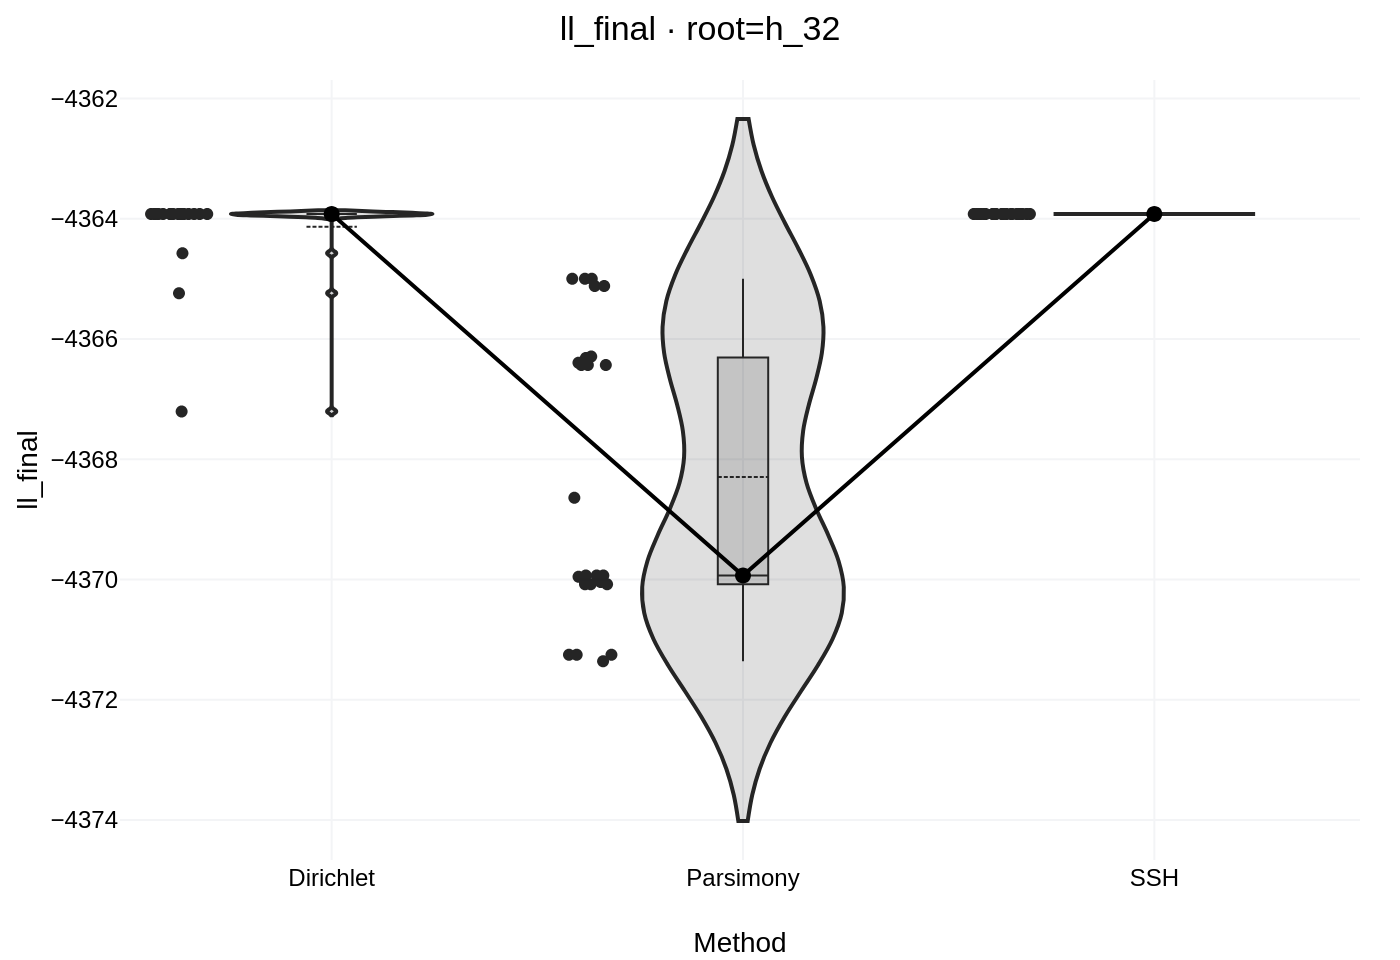
\includegraphics[width=0.8\textwidth]{"/home/pk/projects/prabhavk.github.io/public/figures/wasm-1756002951415__violin__ll_final_violin__t20250824_225734Z.png"}
			\caption{This is the caption describing the figure.}
			\label{fig:my_label}
		\end{figure}
		
		\subsection{Distribution of optimization scores across root locations}
		\begin{figure}[htbp]
			\centering
			\includegraphics[width=0.8\textwidth]{path/to/your/figure.png}
			\caption{This is the caption describing the figure.}
			\label{fig:my_label}
		\end{figure}
		
		\subsection{Wilcoxon-Mann-Whitney tests for difference in log likelihood scores}
			\subsubsection{Impact on initialization method}
			\subsubsection{Impact on root location}
			\begin{table}[htbp]
				\centering
				\small
				\setlength{\tabcolsep}{4pt}
				\renewcommand{\arraystretch}{1.1}
				\begin{tabular}{l*{17}{c}}
					\toprule
					row $\downarrow$ / col $\rightarrow$
					& h\_21 & h\_22 & h\_23 & h\_24 & h\_25 & h\_26 & h\_27 & h\_28 & h\_29 & h\_30 & h\_31 & h\_32 & h\_33 & h\_34 & h\_35 & h\_36 & h\_37 \\
					\midrule
					\textit{sample size (per node)}
					& 30 & 30 & 30 & 30 & 30 & 30 & 30 & 30 & 30 & 30 & 30 & 30 & 30 & 30 & 30 & 30 & 30 \\
					\midrule
					h\_21 & \textemdash & 2 & 3 & 3 & 3 & 3 & 3 & 2 & 2 & 3 & 2 & 3 & 3 & 3 & 3 & 3 & 0 \\
					h\_22 & 1 & \textemdash & 3 & 3 & 3 & 3 & 3 & 2 & 2 & 3 & 1 & 3 & 3 & 3 & 3 & 3 & 0 \\
					h\_23 & 0 & 0 & \textemdash & 3 & 3 & 3 & 3 & 1 & 2 & 1 & 0 & 3 & 3 & 3 & 3 & 3 & 0 \\
					h\_24 & 0 & 0 & 0 & \textemdash & 3 & 3 & 3 & 0 & 2 & 0 & 0 & 3 & 3 & 3 & 3 & 1 & 0 \\
					h\_25 & 0 & 0 & 0 & 0 & \textemdash & 3 & 0 & 0 & 0 & 0 & 0 & 3 & 1 & 1 & 1 & 1 & 0 \\
					h\_26 & 0 & 0 & 0 & 0 & 0 & \textemdash & 0 & 0 & 0 & 0 & 0 & 3 & 1 & 1 & 1 & 1 & 0 \\
					h\_27 & 0 & 0 & 0 & 0 & 3 & 3 & \textemdash & 0 & 2 & 0 & 0 & 3 & 3 & 3 & 3 & 1 & 0 \\
					h\_28 & 1 & 1 & 2 & 3 & 3 & 3 & 3 & \textemdash & 3 & 3 & 1 & 3 & 3 & 3 & 3 & 3 & 0 \\
					h\_29 & 1 & 1 & 1 & 1 & 3 & 3 & 1 & 0 & \textemdash & 1 & 0 & 3 & 3 & 3 & 1 & 1 & 0 \\
					h\_30 & 0 & 0 & 2 & 3 & 3 & 3 & 3 & 0 & 2 & \textemdash & 0 & 3 & 3 & 3 & 3 & 3 & 0 \\
					h\_31 & 1 & 2 & 3 & 3 & 3 & 3 & 3 & 2 & 3 & 3 & \textemdash & 3 & 3 & 3 & 3 & 3 & 1 \\
					h\_32 & 0 & 0 & 0 & 0 & 0 & 0 & 0 & 0 & 0 & 0 & 0 & \textemdash & 1 & 0 & 0 & 1 & 0 \\
					h\_33 & 0 & 0 & 0 & 0 & 2 & 2 & 0 & 0 & 0 & 0 & 0 & 2 & \textemdash & 0 & 0 & 1 & 0 \\
					h\_34 & 0 & 0 & 0 & 0 & 2 & 2 & 0 & 0 & 0 & 0 & 0 & 3 & 3 & \textemdash & 0 & 1 & 0 \\
					h\_35 & 0 & 0 & 0 & 0 & 2 & 2 & 0 & 0 & 2 & 0 & 0 & 3 & 3 & 3 & \textemdash & 1 & 0 \\
					h\_36 & 0 & 0 & 0 & 2 & 2 & 2 & 2 & 0 & 2 & 0 & 0 & 2 & 2 & 2 & 2 & \textemdash & 0 \\
					h\_37 & 3 & 3 & 3 & 3 & 3 & 3 & 3 & 3 & 3 & 3 & 2 & 3 & 3 & 3 & 3 & 3 & \textemdash \\
					\bottomrule
				\end{tabular}
				\caption{Agreement counts: number of methods supporting column $>$ row for each node pair.}
				\label{tab:wmw_agreement}
			\end{table}
			
		\subsection{Significance of recall values}
		
	\section{Methods}		
		\subsection{EM for fixed topology and root}
		\subsection{Parameter initialization}
		\subsubsection{Dirichlet}
		\subsubsection{Parsimony}
		\subsubsection{SSH}
		\subsection{Statistical tests}
		\subsection{Reproducibility of results}
	\section{Discussion}	
	
\end{document}


